%%%%%%%%%%%%%%%%%%%%%%%%%%%%%%%%%%%%%%%%%
% Arsclassica Article
% LaTeX Template
% Version 1.1 (1/8/17)
%
% This template has been downloaded from:
% http://www.LaTeXTemplates.com
%
% Original author:
% Lorenzo Pantieri (http://www.lorenzopantieri.net) with extensive modifications by:
% Vel (vel@latextemplates.com)
%
% License:
% CC BY-NC-SA 3.0 (http://creativecommons.org/licenses/by-nc-sa/3.0/)
%
%%%%%%%%%%%%%%%%%%%%%%%%%%%%%%%%%%%%%%%%%

%----------------------------------------------------------------------------------------
%	PACKAGES AND OTHER DOCUMENT CONFIGURATIONS
%----------------------------------------------------------------------------------------

\documentclass[
10pt, % Main document font size
a4paper, % Paper type, use 'letterpaper' for US Letter paper
oneside, % One page layout (no page indentation)
%twoside, % Two page layout (page indentation for binding and different headers)
headinclude,footinclude, % Extra spacing for the header and footer
BCOR5mm, % Binding correction
]{scrartcl}


%----------------------------------------------------------------------------------------
%	REQUIRED PACKAGES
%----------------------------------------------------------------------------------------

\usepackage[
nochapters, % Turn off chapters since this is an article        
beramono, % Use the Bera Mono font for monospaced text (\texttt)
eulermath,% Use the Euler font for mathematics
pdfspacing, % Makes use of pdftex’ letter spacing capabilities via the microtype package
dottedtoc % Dotted lines leading to the page numbers in the table of contents
]{classicthesis} % The layout is based on the Classic Thesis style

\usepackage{arsclassica} % Modifies the Classic Thesis package

\usepackage[T1]{fontenc} % Use 8-bit encoding that has 256 glyphs

\usepackage[utf8]{inputenc} % Required for including letters with accents

\usepackage{graphicx} % Required for including images
\graphicspath{{Figures/}} % Set the default folder for images

\usepackage{enumitem} % Required for manipulating the whitespace between and within lists

\usepackage{lipsum} % Used for inserting dummy 'Lorem ipsum' text into the template

\usepackage{subfig} % Required for creating figures with multiple parts (subfigures)

\usepackage{amsmath,amssymb,amsthm} % For including math equations, theorems, symbols, etc

\usepackage{varioref} % More descriptive referencing

\usepackage[german]{babel}

\usepackage{tabularx}

% listings
\usepackage{listings}

\lstdefinestyle{mStyle}{
    basicstyle=\linespread{1.0}\normalsize\ttfamily,
    keepspaces=false,
    keywordstyle=\color{Fuchsia},
    identifierstyle=\color{MidnightBlue},
    commentstyle=\color{Green},
    stringstyle=\color{Mahogany},
    columns=flexible
}

%----------------------------------------------------------------------------------------
%	THEOREM STYLES
%---------------------------------------------------------------------------------------

\theoremstyle{definition} % Define theorem styles here based on the definition style (used for definitions and examples)
\newtheorem{definition}{Definition}

\theoremstyle{plain} % Define theorem styles here based on the plain style (used for theorems, lemmas, propositions)
\newtheorem{theorem}{Theorem}

\theoremstyle{remark} % Define theorem styles here based on the remark style (used for remarks and notes)

%----------------------------------------------------------------------------------------
%	HYPERLINKS
%---------------------------------------------------------------------------------------

\hypersetup{
%draft, % Uncomment to remove all links (useful for printing in black and white)
colorlinks=true, breaklinks=true, bookmarks=true,bookmarksnumbered,
urlcolor=webbrown, linkcolor=RoyalBlue, citecolor=webgreen, % Link colors
pdftitle={}, % PDF title
pdfauthor={\textcopyright}, % PDF Author
pdfsubject={}, % PDF Subject
pdfkeywords={}, % PDF Keywords
pdfcreator={pdfLaTeX}, % PDF Creator
pdfproducer={LaTeX with hyperref and ClassicThesis} % PDF producer
} % Include the structure.tex file which specified the document structure and layout

\hyphenation{Fortran hy-phen-ation} % Specify custom hyphenation points in words with dashes where you would like hyphenation to occur, or alternatively, don't put any dashes in a word to stop hyphenation altogether

%----------------------------------------------------------------------------------------
%	TITLE AND AUTHOR(S)
%----------------------------------------------------------------------------------------

\title{\normalfont\spacedallcaps{Pic-Simulator Dokumentation}} % The article title

%\subtitle{Subtitle} % Uncomment to display a subtitle

\author{\spacedlowsmallcaps{David Schmidt \& Moritz Knapp}} % The article author(s) - author affiliations need to be specified in the AUTHOR AFFILIATIONS block

\date{} % An optional date to appear under the author(s)

%----------------------------------------------------------------------------------------

\begin{document}

%----------------------------------------------------------------------------------------
%	HEADERS
%----------------------------------------------------------------------------------------

\renewcommand{\sectionmark}[1]{\markright{\spacedlowsmallcaps{#1}}} % The header for all pages (oneside) or for even pages (twoside)
%\renewcommand{\subsectionmark}[1]{\markright{\thesubsection~#1}} % Uncomment when using the twoside option - this modifies the header on odd pages
\lehead{\mbox{\llap{\small\thepage\kern1em\color{halfgray} \vline}\color{halfgray}\hspace{0.5em}\rightmark\hfil}} % The header style

\pagestyle{scrheadings} % Enable the headers specified in this block

%----------------------------------------------------------------------------------------
%	TABLE OF CONTENTS & LISTS OF FIGURES AND TABLES
%----------------------------------------------------------------------------------------

\maketitle % Print the title/author/date block

\setcounter{tocdepth}{2} % Set the depth of the table of contents to show sections and subsections only

\tableofcontents % Print the table of contents

\listoffigures % Print the list of figures

\newpage % Start the article content on the second page, remove this if you have a longer abstract that goes onto the second page

%----------------------------------------------------------------------------------------
%	INTRODUCTION
%----------------------------------------------------------------------------------------

\section{Allgemeines}

\subsection{Simulator im Allgemeinen}
	Grundsätzlich spricht man bei einer Simulation über die möglichst realitätsnahe Nachbildung von Geschehnissen aus der Wirklichkeit. Durch Simulationen können Erkenntnisse über das reale System gewonnen werden. Das simulierende Gerät wird als Simulator bezeichnet. Es dient dazu aus beispielsweise Kosten- oder Sicherheitsgründen sich von der Realität zu lösen, um diese abstrakt zu behandeln. Dadurch wird ein Modell zum experimentieren geschaffen, um die Ergebnisse anschließend auf das reale Problem zu übertragen. In unserem Fall galt es, einen Simulator für den PIC-16F84 zu implementieren. Damit werden Assembler-Programme getestet, bevor sie auf der echten Hardware gestartet werden.
	
	Der signifikante Vorteil einer Simulation ist, dass nichts kaputt gehen kann. Dadurch haben Fehler keine Auswirkungen auf die Realität, und können in dieser aufgrund von Erfahrung vermieden werden. Wichtig zu erwähnen ist dabei, dass nicht jedes Modell perfekt ist. Verlässt man sich zu sehr darauf, dass sich reale Zusammenhänge so verhalten wie in einer Simulation, können unerwartete Reaktionen auf Handlungen folgen.
	
	Ungeachtet dessen, bieten Simulationen eine Grundlage als Entscheidungsbasis für Realisierungen. Dadurch können Probleme frühzeitig erkannt, und vermieden werden.
\subsection{Der Pic-Simulator}
	\subsubsection{Features}
		Folgende Anforderungen an den PIC-Simulator wurden implementiert:
			\begin{itemize}
				\item Die einfachen Literalbefehle, u.a. MOVLW, ADDLW, SUBLW,
				\item u.a. CALL, GOTO (vereinfacht, ohne Rücksicht auf PCLATH),
				\item u.a. MOVWF, MOVF, SUBWF (nur direkte Adressierung, aber mit d-Bit Auswertung),
				\item u.a. DCFSZ, INCFSZ, RLF RRF (nur direkte Adressierung, aber mit d-Bit Auswert.) ,
				\item u.a. BSF, BCF, BTFSC, BTFSS (direkt und indirekt Adressierung) ,
				\item u.a. Bytebefehle, (direkte und indirekte Adressierung),
				\item Timerfunktion mit / ohne Berücksichtigung der Bits im OPTION-Register,
				\item Interrupt für Timer 0,
				\item Interrupt für INT (RB0),
				\item Interrupt für RB4-RB7,
				\item ADDWF PCL mit Berücksichtigung von PCLATH,
				\item I/O Ausgangslatch (Wirkung TRIS-Register auf Ausgangstreiber),
				\item Breakpoints,
				\item Laufzeitzähler (visualisiert),
				\item Stimulation der I/O-Pins per Maus (Toggle-Funktion) ,
				\item Frei wählbare Quarzfrequenz (im Zusammenhang mit dem Laufzeitzähler),
				\item Markieren des aktuellen (nächsten) Befehls im LST-Fenster,
				\item und Fenster für LST, SFR und GPR.
			\end{itemize}
		Lauflicht und Leuchtband können trotz fehlender Hardwareansteuerung simuliert werden, da anhand der Farbe der Buttons zu erkennen ist, welcher sich im aktiven Zustand befindet.
		
	\subsubsection{Benutzeroberfläche}
	Die hier dokumentierte Implementierung des Simulators bietet dem Nutzer eine umfangreiche Bedienungsoberfläche:
	
	\begin{figure}[h]
		\begin{center}
			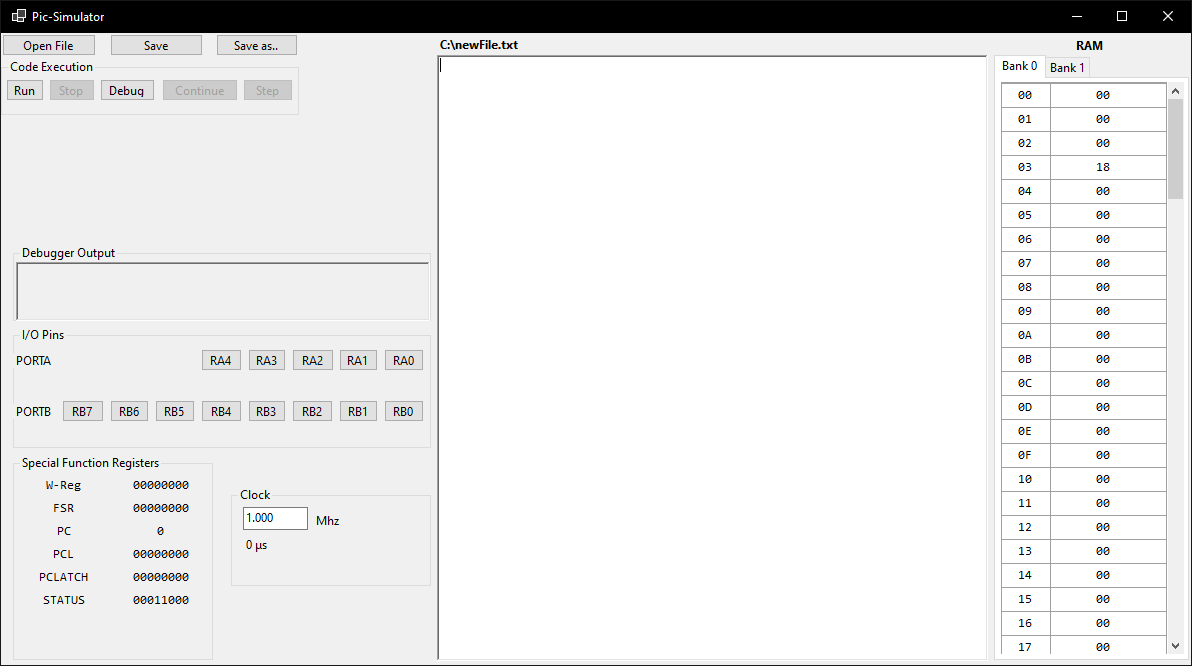
\includegraphics[width=12cm]{GUI.PNG}
			\caption{Benutzeroberfläche}
		\end{center}
	\end{figure}
	
	Neben allgemein bekannten Aktionen von Computerprogrammen (Datei öffnen, Speichern, etc.) finden sich in der oberen linken Ecke Knöpfe, um den Programmablauf zu steuern:
	\begin{figure}[h]
		\begin{tabularx}{\textwidth}{X|X}
			Run			& Die Code-Ausführung wird gestartet. Gesetzte Breakpoints werden dabei ignoriert.		\\
			\hline
			Stop		& Die Code-Ausführung wird gestoppt. Speicherbänke und Register können zwar noch eingelesen werden, sind aber im Hintergrund bereits gelöscht, da das Beenden die Daten des Pics resettet.		\\
			\hline
			Debug		& Hierbei wird eine Code-Ausführung gestartet, welche an gesetzten Breakpoints unterbricht. Ist das Debugging unterbrochen, kann das Programm mit Continue oder Step fortgesetzt werden.		\\
			\hline
			Continue	& Nach einem Stopp wird das Programm fortgesetzt, bis es wieder an einen Breakpoint gelangt.		\\
			\hline
			Step		& Der aktuell markierte Befehl wird ausgeführt und die Markierung springt auf den Befehl, der als nächstes ausgeführt werden würde.		\\
		\end{tabularx}
	\end{figure}

	Darunter befinden sich Ausgabefenster, die I/O-Pins, Special-Function-Register und Timer.
	\\Im Ausgabefenster wird dem Benutzer Rückmeldung zur aktuellen Ausführung des Simulators gegeben, z.B. "Debugging startet". Die darunter liegenden Pins können alle einzeln per Mausklick in den aktiven/inaktiven Zustand versetzt werden, sofern sie als Eingang arbeiten. Sind sie als Ausgang eingestellt, ist an der Farbe zu erkennen, was für ein Pegel (grün = 5V / rot = 0V) gerade anliegt.
	
	Unten links können im SFR-Bereich die wichtigen Register einzeln eingesehen werden. Wichtig dabei ist, dass es sich beim PC lediglich um eine Anzeige handelt, welche keinen Einfluss auf PCLATCH hat. \\Rechts daneben ist angegeben, wie lange das Programm im aktuellen Zustand auf einem PIC gebraucht hätte. Die Quarzfrequenz kann hierbei, auch während des Debuggens, eingestellt werden. 
	
	In der Mitte des Fensters befindet sich der Editor für die Code-Listings. Hier kann der Code textuell bearbeitet werden. Ebenfalls wird immer die Zeile des als nächstes auszuführenden Befehls grün gefärbt. Durch Doppelklicken einer Zeile wird diese als Breakpoint markiert, sofern in dieser Zeile ein Befehl steht. \\
	Auf der rechten Seite sind beide Speicherbänke des Pics dargestellt. Es kann zwischen der Anzeige von Bank 1 und Bank 2 gewechselt werden. 

\section{Realisation}
	\subsection{Grundkonzept}
		Die erste Idee war, den PIC virtuell als Klassenstruktur nachzubauen. Später sollte dann ein Objekt dieses PIC's generiert werden, welches das angegebene Assembler-Programm ausführt. Gleichzeitig sollten auf der Benutzeroberfläche aktuelle Werte der einzelnen Bausteine (RAM, W-Register, etc.) angezeigt werden. Folgende Grafik zeigt das erste Konzept für die eben erwähnte Klassenstruktur:
		\vspace{1cm}
		
		\begin{figure}[h]
			\begin{center}
				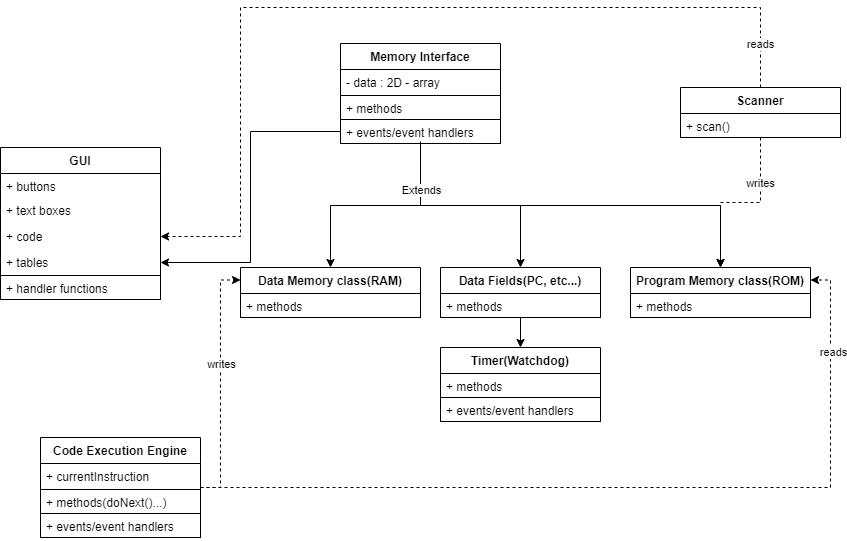
\includegraphics[width=13cm]{ClassDiagram.png}
				\caption{Erstes Klassendiagramm für den Pic}
			\end{center}
		\end{figure}
	
		Zu erkennen ist der Gedanke, dass eine Code-Execution-Engine (untere linke Ecke) den Programmspeicher ausliest und in die Data-Memory schreibt. Die Befehle sollten in der Execution-Engine verarbeitet werden, worauf die richtige Veränderung der Speicherfelder erfolgt. Die Benutzeroberfläche erhält hierbei die benötigten Informationen aus dem Memory-Interface, welches als Elternklasse für alle möglichen Datenspeicher des PIC's (RAM, ROM, PC, W-Reg, etc.) dient.
		
	\subsection{Programmablauf}
		Da die Implementierung der grafischen Benutzeroberfläche wenig bis gar nichts mit der eigentlichen PIC-Simulation zu tun hat, wird in diesem Dokument nicht weiter darauf eingegangen. Der spannende Teil des Programms ist die Ausführung eines Befehls. Es wurde hierbei versucht die Schritte eines realen PIC's bestmöglich nachzusimulieren, d. h. Fetch, Decode und Execute wurden als eigene Funktionen realisiert. Die Code-Ausführung gliedert sich in mehrere Steps. Ein Step führt den aktuell auszuführenden Befehl aus. Folgendes Ablaufdiagramm visualisiert diese Ausführung:
		
		\begin{figure}[h]
			\begin{center}
				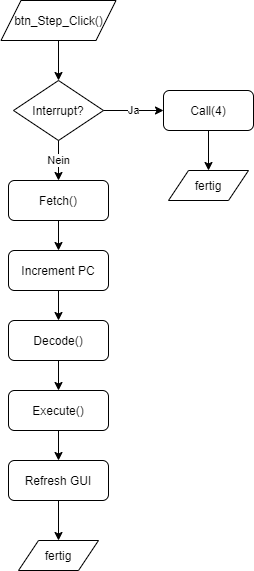
\includegraphics[width=4cm]{StepDiagram.png}
				\caption{Ablaufdiagramm zu einem Step}
			\end{center}
		\end{figure}
	
		Wird auf den Step-Button geklickt, wird ein Step ausgeführt. Dieser überprüft erst, ob zwischen diesem und dem letzten Step ein Interrupt aufgetreten ist. Ist dies der Fall, wird anstelle des eigentlichen Befehls ein Call an Adresse \texttt{4} (ISR) ausgeführt. Wenn nicht, folgt ein Aufruf von \texttt{Fetch}. Genaueres zur Überprüfung von Interrupts ist in \ref{sec:checkInt} aufgeführt. Diese Funktion erhält aus dem Code-Listing den nächst auszuführenden Befehl, um ihn nach Inkrementierung des PC's an \texttt{Decode()} zu übergeben. Anders als bei einem echten PIC ermittelt \texttt{Decode()} lediglich, um was für einen Befehl es sich handelt. \texttt{Execute()} bekommt diesen als eine Instanz der eigens erstellten Enumeration mit zusätzlich allen \texttt{16} Bits des Befehlsaufrufs übergeben und führt ihn aus. Nachdem daraufhin die Benutzeroberfläche alle Elemente und Register aktualisiert hat, kann ein nächster Step durchgeführt werden.
		
	\subsection{Programmiersprache}
		Es wurde sich schnell für die Programmiersprache C\# entschieden. Wir beide haben in unserem Studium gemerkt wie umfangreich Benutzeroberflächenanbindungen sein können. Da dies bei C\# sehr einfach mit Windows-Forms umzusetzen ist, schien die Wahl logisch. Zudem ist die Syntax sehr C-ähnlich. Dadurch konnte viel Zeit gespart werden, da sich keiner von uns in eine neue Sprache einlesen musste.
	\subsection{Evaluierung eines eingehenden Befehls (Decode)}
		Um zu erkennen um welchen Befehl es sich bei der Eingabe handelt, muss dieser von seinen Parametern getrennt werden. Dies wird mit der logischen Verundung der Eingabe und einer Befehlsmaske realisiert. Beispielsweise hat der Befehl DECF folgendes Schema:
		
		\begin{figure}[h]
			\begin{itemize}
				\item DECF: \texttt{0000 0011 dfff ffff}
			\end{itemize}
		\end{figure}
		In diesem Fall geben die f-Bits die Adresse im File-Register an und das d-Bit, wo der Ergebniswert der Operation gespeichert werden soll. Der Befehl selbst wird aber nur innerhalb der ersten 8 Bits dekodiert. Verzichtet man auf die Verundung mit der Maske könnte nicht festgestellt werden, ob es sich bei einem Bit um eine Befehlscodierung oder einen Parameter handelt. Verundet man nun eine Eingabe mit in diesem Fall der Maske \texttt{1111 1111 0000 0000}, entfallen alle nicht-relevanten Bits und es kann festgestellt werden, um welchen Befehl es sich handelt.
	\subsection{Befehle}
		Im Folgenden wird die Realisierung der einzelnen Befehle erläutert. Dazu verschafft ein generelles Ablaufdiagramm einen Überblick zur Befehlsabarbeitung, woraufhin einzelne Befehle beispielhaft erläutert werden.
		\subsubsection{Allgemeiner Ablauf der Befehlsausführung}
		
			\begin{figure}[h]
				\begin{center}
					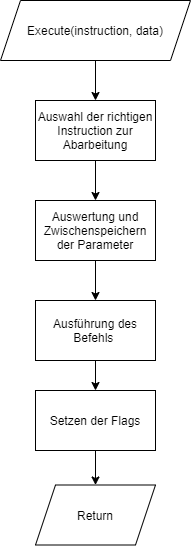
\includegraphics[width=5cm]{BefehlAllg.png}
					\caption{Ablaufdiagramm zur allgemeinen Befehlsabarbeitung}
				\end{center}
			\end{figure}
		
			Die einzelnen Befehlsimplementierungen sind in einem großen Switch-Case-Statement der \texttt{Execute}-Funktion aufgelistet. Als Übergabeparameter erhält sie zum einen die \texttt{instruction<Instruction>} der Enumeration und diese zusätzlich als \texttt{data<UInt16>}. In \texttt{data} sind alle 16 Bit des Befehls enthalten und müssen im 2. Schritt des Ablaufdiagramms befehlsspezifisch in einzelne Variablen zwischengespeichert werden, um diese daraufhin zu verarbeiten.  
			Nach der Ausführung des Befehls (Addition, Bitshifting, Speicherbearbeitung, etc.) werden die richtigen Flags gesetzt, woraufhin \texttt{true} zurückgegeben wird. Gibt es keinen \texttt{case} welcher auf die eingehende \texttt{Instruction} passt, wird \texttt{false} zurückgegeben.
		\newpage
		Um die Implementierung einzelner Befehlsabarbeitungen zu verstehen, müssen folgende Hilfsfunktionen bekannt sein:
		\subsubsection{\texttt{Set()}}
			Diese Funktion kann die folgenden drei Parameter übernehmen:
			
			\begin{figure}[h]
				\begin{itemize}
					\item \texttt{byte adress}: Die Adresse, an die geschrieben werden soll,
					\item \texttt{bool bank}: Eine Angabe der Bank, auf welche zu schreiben ist,
					\item \texttt{byte result}: Der Wert, welcher an die Adresse geschrieben wird.
				\end{itemize}
			\end{figure}
			Die Bank muss nur gegebenenfalls angegeben werden, da sie in den meisten Fällen dem Wert an RP0 entnommen wird.
			\newpage
		\subsubsection{\texttt{GetFlag()}}
			Hier wird der Wert eines einzelnen Bits zurückgegeben. Es wird die Adresse an welcher das Bit gelesen werden soll, sowie der Index des Bits angegeben. Auch hier gibt es eine Überladung, bei der die Bank gegebenenfalls angegeben werden kann. Dies wird später interessant, wenn beispielsweise ein einzelnes Bit aus dem TRIS-Register gelesen werden soll.
			
		\subsubsection{\texttt{Set}- und \texttt{ClearFlag()}}
		\label{sec:setClearFlag}
			Analog zu \texttt{GetFlag} dienen diese Funktionen dazu, ein in den Übergabeparametern spezifiziertes Bit zu Setzen oder Rück- zu setzen. 
			
		\subsubsection{ADDLW}
			Bei dieser Operation ist der Wert des angegebenen Literals dem Wert im W-Register zu addieren.
			In der Implementierung werden als erstes beide Operanden der Addition in separaten Variablen gespeichert. Da es sich bei der Operation um eine Byte-Addition handelt, kann nur mit \texttt{overflowCheck} vom Typ Int festgestellt werden, ob es zu einem Überlauf kam, da Int's auch größere Werte als 255 annehmen können:
			
			\begin{figure}[h]
				\begin{center}
					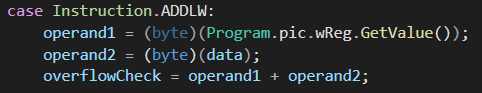
\includegraphics{OpTrennungADDLW.PNG}
					\caption{Operandentrennung bei ADDLW}
				\end{center}
			\end{figure}
		
			Daraufhin wird der Wert des Ergebnisses der Byte-Addition in das W-Register geschrieben:
			
			\begin{figure}[h]
				\begin{center}
					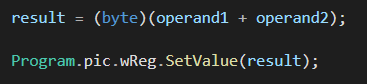
\includegraphics{setWreg.png}
				\end{center}
			\end{figure}
		
			
			Als nächstes ist zu prüfen, wie das Digit-Carry-Flag zu setzen ist. Dazu werden beide Operanden mit einer Maske verundet, sodass nur die ersten 4 Bits Auswirkung auf Operationen haben.  Die Maske dazu ist \texttt{00001111}. Daraufhin kann das Digit-Carry-Flag gesetzt werden, sofern eine Addition dieser verundeten Bytes ein größeres Ergebnis als 15 liefert:
			
			\begin{figure}[h]
				\begin{center}
					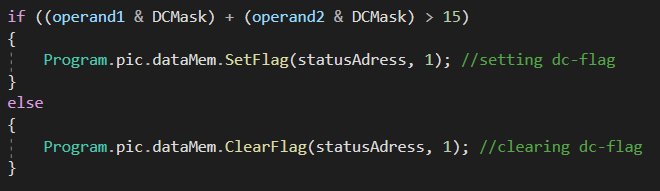
\includegraphics[width=12cm]{dcFlagCheck.png}
					\caption{Überlauf-Check der unteren 4 Bits}
				\end{center}
			\end{figure}
		
			Mit den bereits in \ref{sec:setClearFlag} erklärten Funktionen kann daraufhin das Digit-Carry-Flag richtig gesetzt werden. \\
			Nun Fehlen noch die Auswirkungen auf Carry-Flag und Zero-Flag.
			Ähnlich wie beim Digit-Carry-Flag ist hier zu überprüfen, ob das Ergebnis größer als \texttt{255} ist und dementsprechend die Flag richtig zu setzen:
			
			\begin{figure}[h]
				\begin{center}
					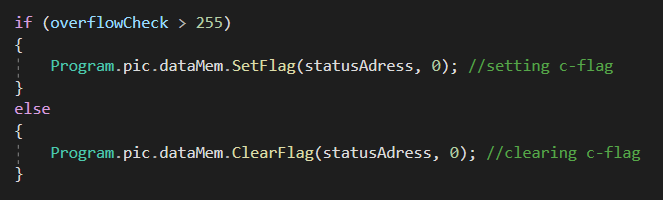
\includegraphics[width=\textwidth]{setClearCFlag.png}
					\caption{Überlauf-Check der Byte-Addition}
				\end{center}
			\end{figure}
		
			Auf gleiche Weise wird überprüft, ob das Ergebnis den Wert \texttt{0} hat, und dementsprechend die Zero-Flag gesetzt. Zusätzlich gibt es bei diesem Befehl noch eine weitere Abfrage, da sowohl Digit-Carry als auch Carry rückgesetzt werden müssen, sofern der zweite Operand den Wert \texttt{0} hat.
			
			
	\subsection{Check Interrupt}
	\label{sec:checkInt}
		Der erste Schritt ist die Überprüfung von \texttt{Global Interrupt Enable Flag} (INTCON, 7). Falls dies gesetzt ist, werden nacheinander die spezifischen Interrtupt-Flags (INTCON 3-5) überprüft. Falls eine entsprechende Flag gesetzt ist, wird die Interrupt-Methode aufgerufen, welche das \texttt{Global Interrupt Enable Flag} rücksetzt und die Interrupt Service Routine aufruft (CALL(4)).
		\texttt{CheckInterrupt()} ist in folgendem Listing dargestellt:
		
		\begin{figure}[h]
			\begin{center}
				\includegraphics[width=\textwidth]{CheckInterrupt.PNG}
				\caption{\texttt{CheckInterrupt()}}
			\end{center}
		\end{figure}
	\newpage
	\subsection{Wirkung des Tris-Registers auf den Ausgangstreiber}
		Ob ein Port als Ausgang oder Eingang arbeitet, ist durch seine Klickbarkeit gekennzeichnet. D.h. wenn man einen der Ports anklicken kann, arbeitet dieser als Eingang. Im Code gibt es eine Funktion Namens \texttt{UpdatePortButtons()}. Diese iteriert durch alle Port-Buttons und prüft dabei, ob das entsprechende Bit im passenden Tris-Register gesetzt ist. Ist dies der Fall, wird \texttt{Button.enabled} auf true gesetzt, da er als Eingang arbeitet und somit geklickt werden kann.
		Dieser Vorgang findet statt, nachdem auf ähnliche Weise die Hintergrundfarbe entsprechend der Bits im Portregister eingestellt wurde. Das folgende Code-Beispiel zeigt diese Implementierung für die RA-Ports:
		
		\begin{figure}[h]
			\begin{center}
				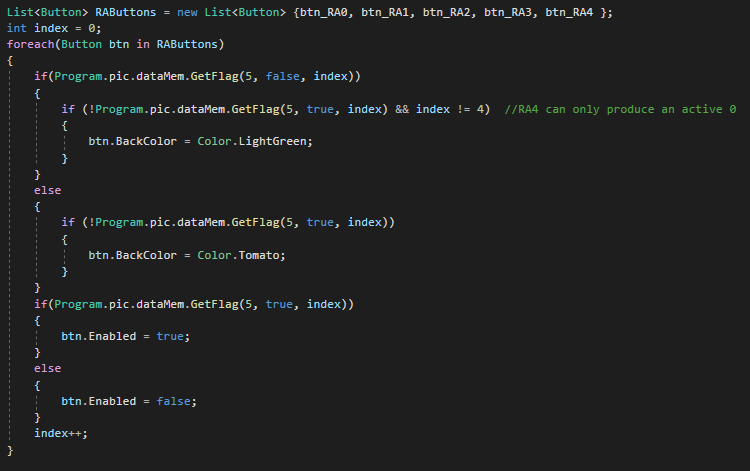
\includegraphics[width=\textwidth]{UpdatePorts.png}
				\caption{Update der Port-Buttons für RA}
			\end{center}
		\end{figure}
		
		Ebenfalls ist hier zu erkennen, dass die Variable \texttt{index} immer auf den aktuell zu behandelnden Port deutet. Dadurch kann beispielsweise verhindert werden, dass RA4 eine aktive \texttt{1} erzeugt.
		\newpage
\section{Zusammenfassung}
	\subsection{Bewertung der virtuellen Nachbildung des PICs}
		Wie bereits erwähnt, war die Grundidee dieser Simulation den PIC virtuell nachzubauen. Dabei musste für die Nachbildung eine Abstraktion des PICs durchgeführt werden. Anderenfalls müsste beispielsweise die Funktionsweise einzelner Hardwarebausteine, wie Transistoren, Logikgatter oder dergleichen, nachgebildet werden um einen "richtig echten" PIC virtuell zu nachzustellen. Wichtig war uns, dass wir trotz Abstraktion die Grundbausteine wie RAM, W-Register, etc. als getrennte Klassen implementieren. So konnte ein PIC erstellt werden bei dem bei Initialisierung klar zu erkennen ist, aus welchen Teilen er besteht:
		
		\begin{figure}[h]
			\begin{center}
				\includegraphics[width=11cm]{PICIni.png}
				\caption{PIC-Initialisierung}
			\end{center}
		\end{figure}
		
		Befehlsausführungen haben abstrakte Vorgänge eines realen PICs in ihrer Funktion nachgebildet. Das bedeutet, dass die einzelnen Schritte auf der Hardware von beispielsweise MOVLW virtuell nicht stattfinden, das Literal jedoch trotzdem in einer Instanz: "W-Register" gespeichert wird. Unserer Meinung nach reicht dieser Sachverhalt dennoch aus, um den PIC-Simulator als "realitätsnah" zu bezeichnen. Wäre tatsächlich auch die Hardware nachgebildet, wäre das Ergebnis eines Programms trotzdem das gleiche.  
		\newpage
	\subsection{Fazit}
		Grundsätzlich lässt sich sagen, dass die Zusammenarbeit als Team sehr gut funktioniert hat. Wir teilten uns zu Beginn der Programmierung auf und jeder hat eigenständig Teile des PICs implementiert, die von einander abhängig sind und zusammen arbeiten. Als wir nach einigen Tagen das erste Mal die Ausführung einfache Literalbefehle ausprobierten, war dieser erste Test zu unserer Überraschung erfolgreich. Daraufhin vielen Sätze wie "Die Teamarbeit hat ja mal mega gut geklappt", wodurch die Motivation für das Projekt extrem gesteigert wurde. Generell bereitete uns das Arbeiten am PIC-Simulator viel Freude.\\
		Wir erkannten schnell dass uns das Thema dieses Projekts sehr interessiert hat. Ebenfalls handelte es sich um unsere erste Zusammenarbeit für ein doch relativ umfangreiches Softwareprojekt. Dass, wie eben erwähnt, die Stimmung bei der Arbeit ausgesprochen gut war, wirkte sich sehr positiv auf die Produktivität und Eigeninitiative aus.\\
		Wichtig zu erwähnen ist an dieser Stelle auch, dass wir beide während des Projektes sehr viel über den PIC gelernt haben. Ohne ein genaues Verständnis über das Verhalten einzelner Befehle wäre eine genaue Nachbildung nicht möglich. Sein es die Ausführung einzelner Befehle, das Verhalten des Stacks oder auch komplexere Abläufe wie Timer oder Interrupt, alles musste genauestens erlernt werden. Logischerweise führte übermotiviertes Losprogrammieren zu falschen Ansätzen, die nach Recherche über den PIC überarbeitet werden mussten. Mit unserem jetzigen Kenntnisstand könnte ein Simulator also wesentlich schneller programmiert werden. \\
		Zusammenfassend lässt sich also sagen, dass die Stimmung während der Programmierung sehr gut war. Wir beide lernten sehr viel über den PIC und arbeiteten mit Freude an diesem Projekt. Im Nachhinein würden wir allerdings einige Dinge von vornherein anders planen, wodurch viel Zeit gespart würde.
%------------------------------------------------


%----------------------------------------------------------------------------------------
%	BIBLIOGRAPHY
%----------------------------------------------------------------------------------------

\renewcommand{\refname}{\spacedlowsmallcaps{References}} % For modifying the bibliography heading

\bibliographystyle{unsrt}

\bibliography{sample.bib} % The file containing the bibliography

%----------------------------------------------------------------------------------------

\end{document}